\documentclass{article}

\title{P01-Compression  Report}
\date{13/10/2017}
\author{150008859}

\setlength{\parskip}{1em}
\setlength{\parindent}{0em}

\usepackage{listings}
\usepackage{amsmath,amssymb,amsthm}
\usepackage{mathtools}
\usepackage{graphicx}


\begin{document}
\maketitle
\newpage

\section{Introduction}

This practical involved writing an application to be able to experiment with Huffman and Arithmetic coding. In this report, I present my findings when comparing Huffman and Arithmetic. In addition, I explain any important design decisions and I present two extensions which include Adaptive Huffman coding and Zip.

\section{Usage}

\subsection{Compiling}

I have included two projects. Both projects use \textbf{ant}.

The one titled P01-Compression has a graphical user interface.

The one titled ZipUtility is a command line tool.

I recommend following the instructions in the order they are given. 

To compile a project, enter its directory. A Build.xml file should be present.

To compile and create a jar file, run the following instructions.
\begin{lstlisting}[language=bash]
  ant clean
  ant compile
  ant jar
\end{lstlisting}

\subsection{Zip Utility}

These are the exact instructions needed to run ZipUtility. 

\begin{lstlisting}[language=bash]
  cd ZipUtility
  ant clean
  ant compile
  ant jar
  java -jar jar/zip.jar res/test2.txt res/test.txt
\end{lstlisting}

The output.zip file should be created containing res/test2.txt and res/text.txt. You can verify that this is a valid zip file by extracting it using another one.


\subsection{P01-Compression}

This has a graphical user interface.

These are the exact instructions needed to run P01-Compression. You should be presented with a GUI.

\begin{lstlisting}[language=bash]
  cd P01-Compression
  ant clean
  ant compile
  ant jar
  ant run
\end{lstlisting}

\begin{figure}[h]
  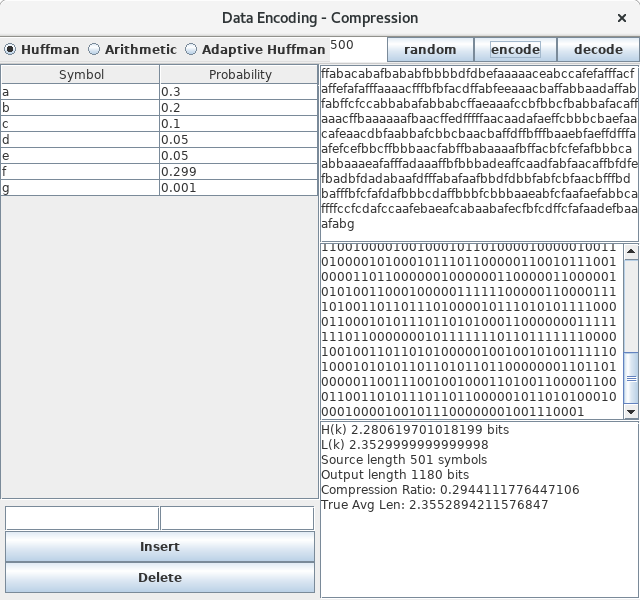
\includegraphics[scale=0.3]{images/gui_b.png}
  \caption{Huffman}
  \label{fig:gui_huffman}
\end{figure}

\begin{figure}
  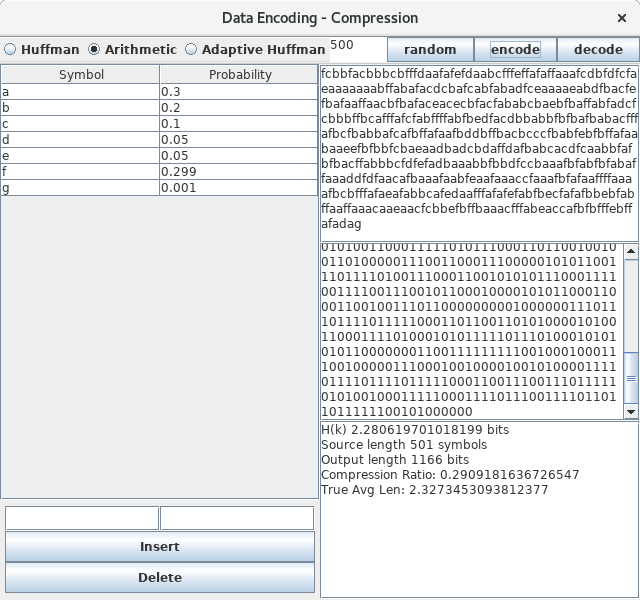
\includegraphics[scale=0.3]{images/gui_c.png}
  \caption{Arithmetic}
  \label{fig:gui_arithetmetic}
\end{figure}

\begin{figure}
  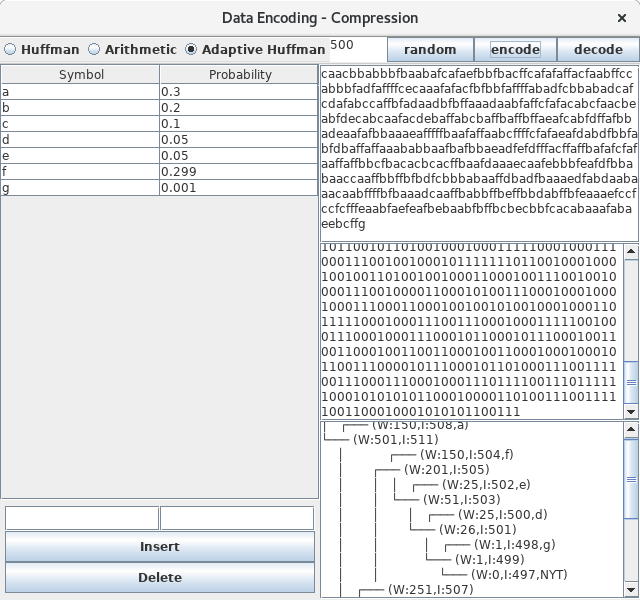
\includegraphics[scale=0.3]{images/gui_d.png}
  \caption{Adaptive Huffman}
  \label{fig:gui_adaptive_huffman}
\end{figure}


\newpage

\begin{lstlisting}[language=bash]

\end{lstlisting}

\begin{verbatim}

\end{verbatim}


\section{Huffman Coding}

\subsection{Introduction}

Huffman Coding is the construction of instaneous coding with guaranteed average minimum length. 

\subsection{Design}

The process begins with a list of leaf nodes containing the symbol and their probability. By sorting the nodes in ascending order, you can collect the two smallest weighted nodes and join to them a parent who's weight is the sum of its children. This parent node replaces the two children in the list. The process is repeated until there is a single node left, this node becomes the root node.

This constructs a Huffman Tree in which the least weighted nodes have the shortest path from the root and hence the shortest code word.

\subsubsection{Encoding}

After the tree is constructed, a depth first search is performed to collect a list of all the leaf nodes. To find a given code word, you can traverse a tree updwards to the root. If the current node is a left child, you append a 1, otherwise if its a right child you append a 0. This string is reversed since the tree was ascended. Doing this for every leaf node, a lookup table is constructed mapping symbol to its code word.

To encode, we can simply map each symbol to its code word using the lookup table and concatenate them all.

\subsubsection{Decoding}

Starting from the root node in the Huffman Tree, if we see a 0 we traverse left, otherwise right for a 1. By following this process, when we reach a leaf node we have successfully decoded a symbol and we can repeat this starting again from the root node to decode the remaining encoded message. We can also determine if something is not decodable if the node we need to traverse to does not exist.

\section{Arithmetic Coding}

Arithmetic Coding encodes a message into a single number such that $ 0 \leq x < 1 $.

\subsection{Design}

My initial strategy involved using BigDecimal to simply experiment with arithmetic coding. This implementation is complete. Except, there is a huge $O(n)$ memory to store the number and its not possible to stream it. You have to wait for the entire message to be encoded before you can start sending bits.

Hence, I quickly abandoned it and implemented it using the algorithm present in the lecture slides.

Instead of using an expensive arbitrary precision data structure, fixed bit integers are used to represent the upper $u$ and lower bound $l$. The number of bits used to represent $u$ and $l$ depends on the precision and magnitude of the probabilities.

At any given point, we're only dealing with a fixed quantity of bits at any given time. This gives the algorithm a constant memory complexity. The upper bound $u$ is treated as a sequence of 1s followed by an infinite sequence of 1s which haven't been shifted into memory. The lower bound is treated as a sequence of 0s followed by an infinite sequence of 0s which have not been shifted into memory.

Note the terminating symbol is the last symbol in the table.

\subsubsection{Encoding}

Encoding is a process of rescaling l and u where we modify l and u to represent a smaller interval.

Due to the invariant $0 \leq l < u \leq 2^B-1$, it can be determined when the most significant bit becomes unchanging. There are two situations referred to as Case A and Case B.

In Case B, it is not immediately known which side interval $u$ and $l$ lies on around the half way mark. So we increment a variable called $S$.

In Case A, the most significant bits are common and we can immediately transfer the most significant bit followed by $S$ bits of the negation of the most significant bit. To replace the most significant bit that has been transferred, we shift $u$ and $l$ to the left remembering that $u$ has a sequence of infinite 1s after it, of which a single bit is shifted into memory.

At this point the entire message has been encoded into a small interval and finally this process is terminated when the terminating symbol has been encoded. 

\subsubsection{Decoding}

Decoding involves constructing a number called $v$ which represents a fixed region of bits in the source message. Decoding is much simpler than encoding. Determining which interval $v$ lies retrieves the encoded symbol. The upper bound $u$ and lower bound $l$ are updated to this interval. We continue to move through the tag message examining a fixed region bits until we reach the terminating symbol.

\section{Huffman vs Arithmetic}

I compared the average bits per symbol as the entropy is its lower bound and it gives an indication of how compressed a message is.

Both tables are generated using the following information source which have the entropy $H(x) = 2.280$

\begin{center}
  \begin{tabular}{ |c|c|c| } 
    \hline
    Symbol & Probability \\
    \hline
    a & 0.3 \\
    b & 0.2 \\
    c & 0.1 \\
    d & 0.05 \\
    e & 0.05 \\ 
    f & 0.299 \\
    g & 0.001 \\ 
    \hline
  \end{tabular}
\end{center}

The following table shows the average bits per symbol (to 3 d.p.).

\begin{center}
  \begin{tabular}{ |c|c|c|c| } 
    \hline
    Length & Huffman & Arithmetic & Adaptive \\
    \hline
    10 & 2.750 & 3.250 & 7.083 \\ 
    50 & 2.442 & 2.519 & 4.057 \\
    100 & 2.376 & 2.405 & 3.406 \\
    500 & 2.355 & 2.327 & 2.557 \\
    5000 & 2.351 & 2.311 & 2.562 \\
    50000 & 2.350 & 2.310 & 2.700 \\
    \hline
  \end{tabular}
\end{center}

The following table shows the compression ratio between the source message if it was in ascii and the encoded message.

\begin{center}
  \begin{tabular}{ |c|c|c|c| } 
    \hline
    Length & Huffman & Arithmetic & Adaptive \\
    \hline
    10 & 0.344 & 0.406 & 0.906 \\ 
    50 & 0.305 & 0.314 & 0.507 \\
    100 & 0.297 & 0.301 & 0.426 \\
    500 & 0.294 & 0.290 & 0.320 \\
    5000 & 0.294 & 0.289 & 0.320 \\
    50000 & 0.293 & 0.289 & 0.337 \\
    \hline
  \end{tabular}
\end{center}

Initially, for a small source message, it appears as if Huffman Coding provides a lower average bits per symbol. However, as the source message length increases, arithmetic coding quickly seems to give a better compression rate and a smaller average bits per symbol compared to Huffman Coding. Increasing the length shows the limiting behaviour. As the length increases, the average bits per symbol for both Huffman and Arithmetic gets closer to the entropy. Arithmetic seems to be closer to its entropy in general compared to Huffman.

No matter how much the source text is increased, the bits per symbol decreases and gets closer to the entropy but it is always greater than the entropy.

In general, Adaptive Huffman doesn't perform as well, but it reaches almost a similar compression rate of around a $1/3$. I hypothesize that this is because it isn't aware of the true probabilities, but instead it takes into account the frequency of letters that have been seen. At some point in the future, some more commonly occuring symbols might occur less often and some less common symbols might appear more often. This would cause larger code words to be generated for a period of time until the newer frequencies caused the tree to rearrange.

\section{Adaptive Huffman}

Huffman Coding and Arithmetic Coding require knowledge of the frequency of the data before data can be transmitted. In addition, this code book or dictionary must be exchanged so the decoder is capable of decoding the message with the same assumption as the encoder.

Instead of a shared dictionary, Adaptive Huffman Coding solves this by maintaining a shared state. This is updated when a character is sent by the encoder and when an encoded symbol is received by the decoder.

An Adaptive Huffman Tree is used to represent this shared state. A Node contains additional fields including an index number and a weight. A leaf node's weight is the number of times that symbol has been updated. The index is used to impose an ordering, this is called the sibling property in which nodes's weight can be listed left to right in a strictly non-decreasing order. Any Tree that maintains this sibling property is called a Huffman Tree.

During the update, this invariant can be broken. When a node's weight is updated, any nodes above including the parent of this node's weight are incremented. To fix this, the node who's weight broke the condition is swapped with the heaviest weight in it's number class. 

A NYT node, which stands for Not Yet Transmitted, represents a symbol which has not been transmitted. It has a weight of 0 and the lowest index number. The NYT is used to spawn a new node for the newly added symbol. The encoder is aware that the character has not been seen yet so the decoder won't be able to decode it without knowing what the symbol is. In order to deal with this, the code word for the NYT is sent followed by the ascii code for the symbol. This way the decoder can update its shared state. In all further correspondence, when that symbol is seen it will be able to decode it.

In the GUI you can see the tree and follow the update procedure by incrementally adding symbols to the source message.

\section{Zip}

I created a Zip utility which constructs a Zip file. Currently, it posseses no compression which means its resembles a tar file.

This is because I couldn't understand some parts of the deflate algorithm, which is a combination of Huffman and LZ77.

I constructed the zip file using PKWARE's specification. A zip is a binary format. In a Zip file, Each file possesses a local header followed by the contents of the file and an entry in a central directory which stores the offset to locate its local header. You can identify what header you're looking at by observing the header's magic number.

I use ByteBuffer to deal with endianess and byte storage. The Zip file is constructed recursively by concatenating together the ByteBuffer of its components.

The zip file generated can store multiple files. 

\section{Conclusion}

In conclusion, Arithmetic coding provides better long term compression in comparison to Huffman coding. Adaptive Huffman Coding performs slightly worse, in exchange for not having to share dictionaries. I found Arithmetic and Adaptive Huffman are both tricky to implement. Arithmetic coding appears to have some patenting issues, perhaps this is why its not used in compression utilities like gzip or zip. Huffman Coding seems to be best balance of easy to implement and provides a good compression ratio.

\end{document}
